\documentclass[/home/jesse/Analysis/Dissertation/ThesisBuxton.tex]{subfiles}
\begin{document}

\subsection{V0 Purity Estimation}
\label{V0PurEst}

In order to obtain a true and reliable signal, one must ensure good purity of the V0 collection.  The purity of the collection is calculated as:

\begin{equation}
 Purity = \frac{Signal}{Signal + Background}
\label{eqn:Purity}
\end{equation}
To access both the signal and background, the invariant mass distribution (\minv) of all V0 candidates must be constructed immediately before the final invariant mass cut, as shown in Fig. \ref{fig:Purities} for \Lam, \ALam and \Ks candidates in the 0-10\% centrality bin.
Fig. \ref{fig:LamPurity} presents the p$\pi^{-}$ invariant mass distribution showing the \Lam peak, Fig. \ref{fig:ALamPurity} presents the $\bar{\mathrm{p}}\pi^{+}$ invariant mass distribution showing the \ALam peak, and Fig. \ref{fig:K0sPurity} presents the $\pi^{+}\pi^{-}$ invariant mass distribution showing the \Ks peak.

It is vital that this distribution be constructed immediately before the final \minv cut, otherwise it would be impossible to estimate the background.
These distributions are used to calculate the collections' purities (defined in Eq. \ref{eqn:Purity}).
As shown in Figure \ref{fig:Purities}, the background is fit (with a polynomial) outside of the peak region of interest to obtain an estimate for the background within the region.
Within the \minv cut limits, the background is assumed to be the region below the fit while the signal is that above the fit.
The \Lam and \ALam purities were found to be $\approx$ 95\%, and the \Ks purity was found to be $\approx$ 98\%.

\begin{figure}[h!]
  \centering
  %%----start of first subfigure---  
  \subfloat[$\Lambda$ Purity]{
    \label{fig:LamPurity}
    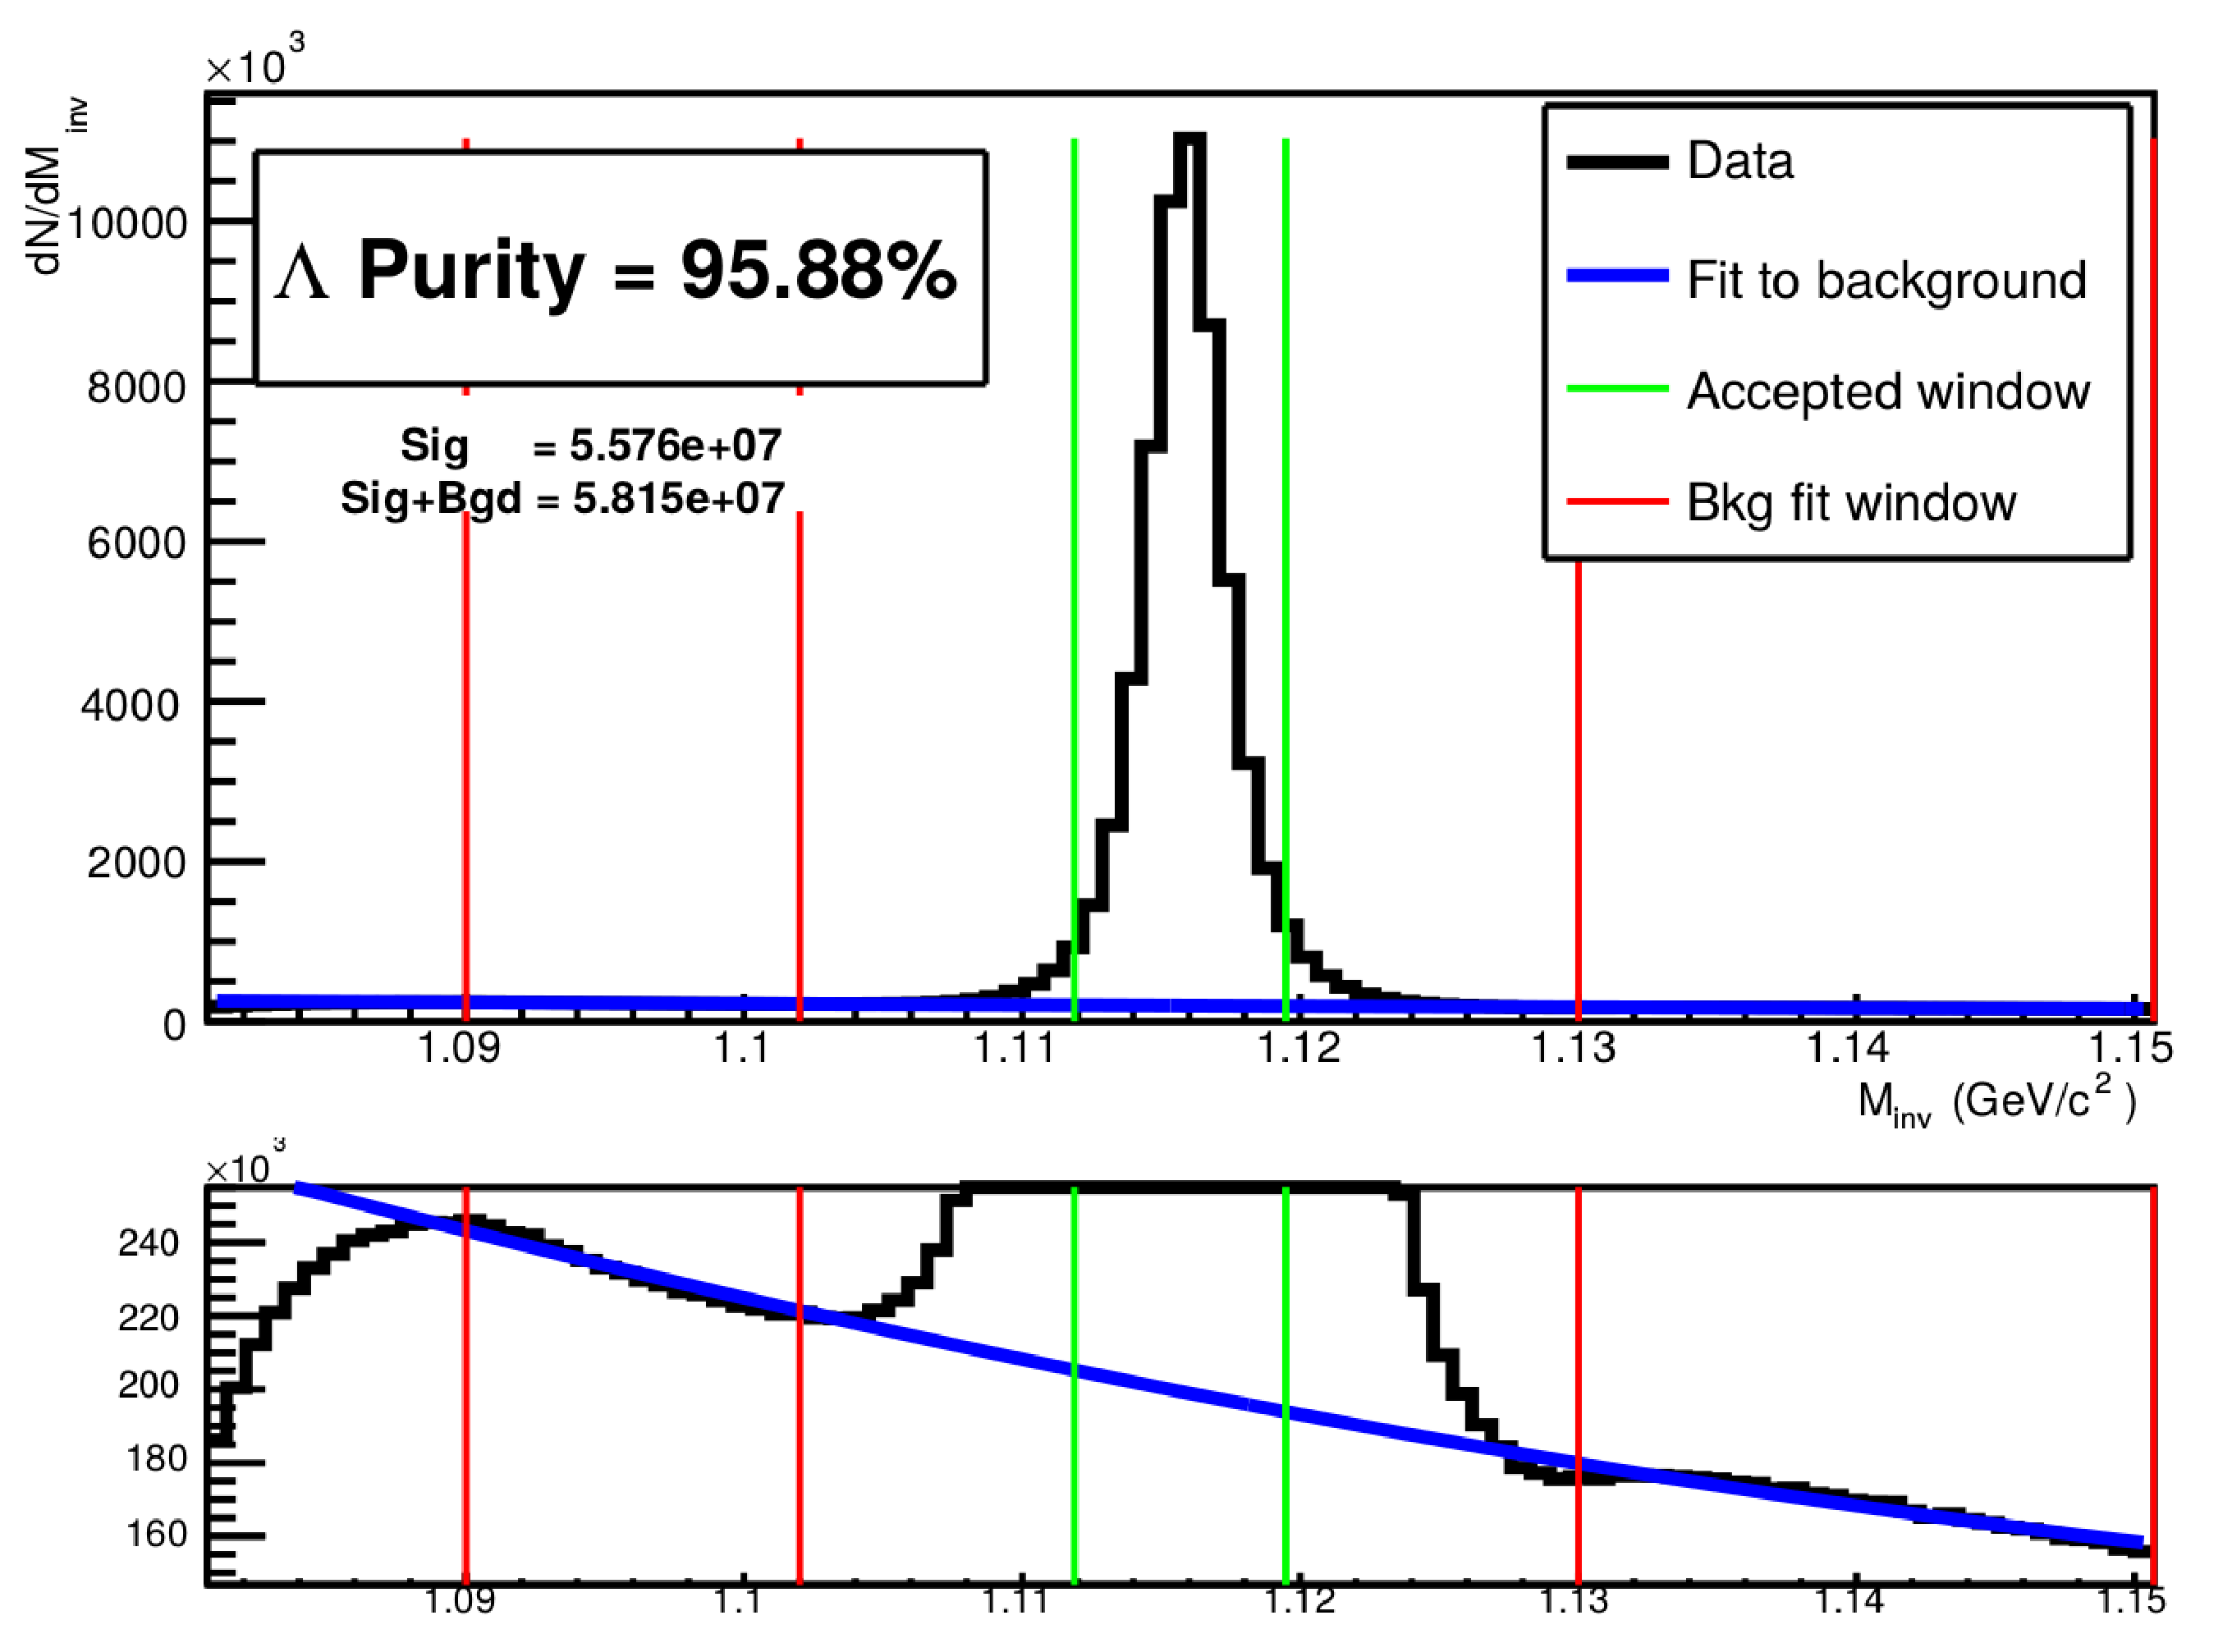
\includegraphics[width=0.49\textwidth]{/home/jesse/Analysis/FemtoAnalysis/AnalysisNotes/3_DataSelection/Figures/LamPurity_LamKch_0010.pdf}}%\\
  %%----start of second subfigure---
  \subfloat[$\bar{\Lambda}$ Purity]{
    \label{fig:ALamPurity}
    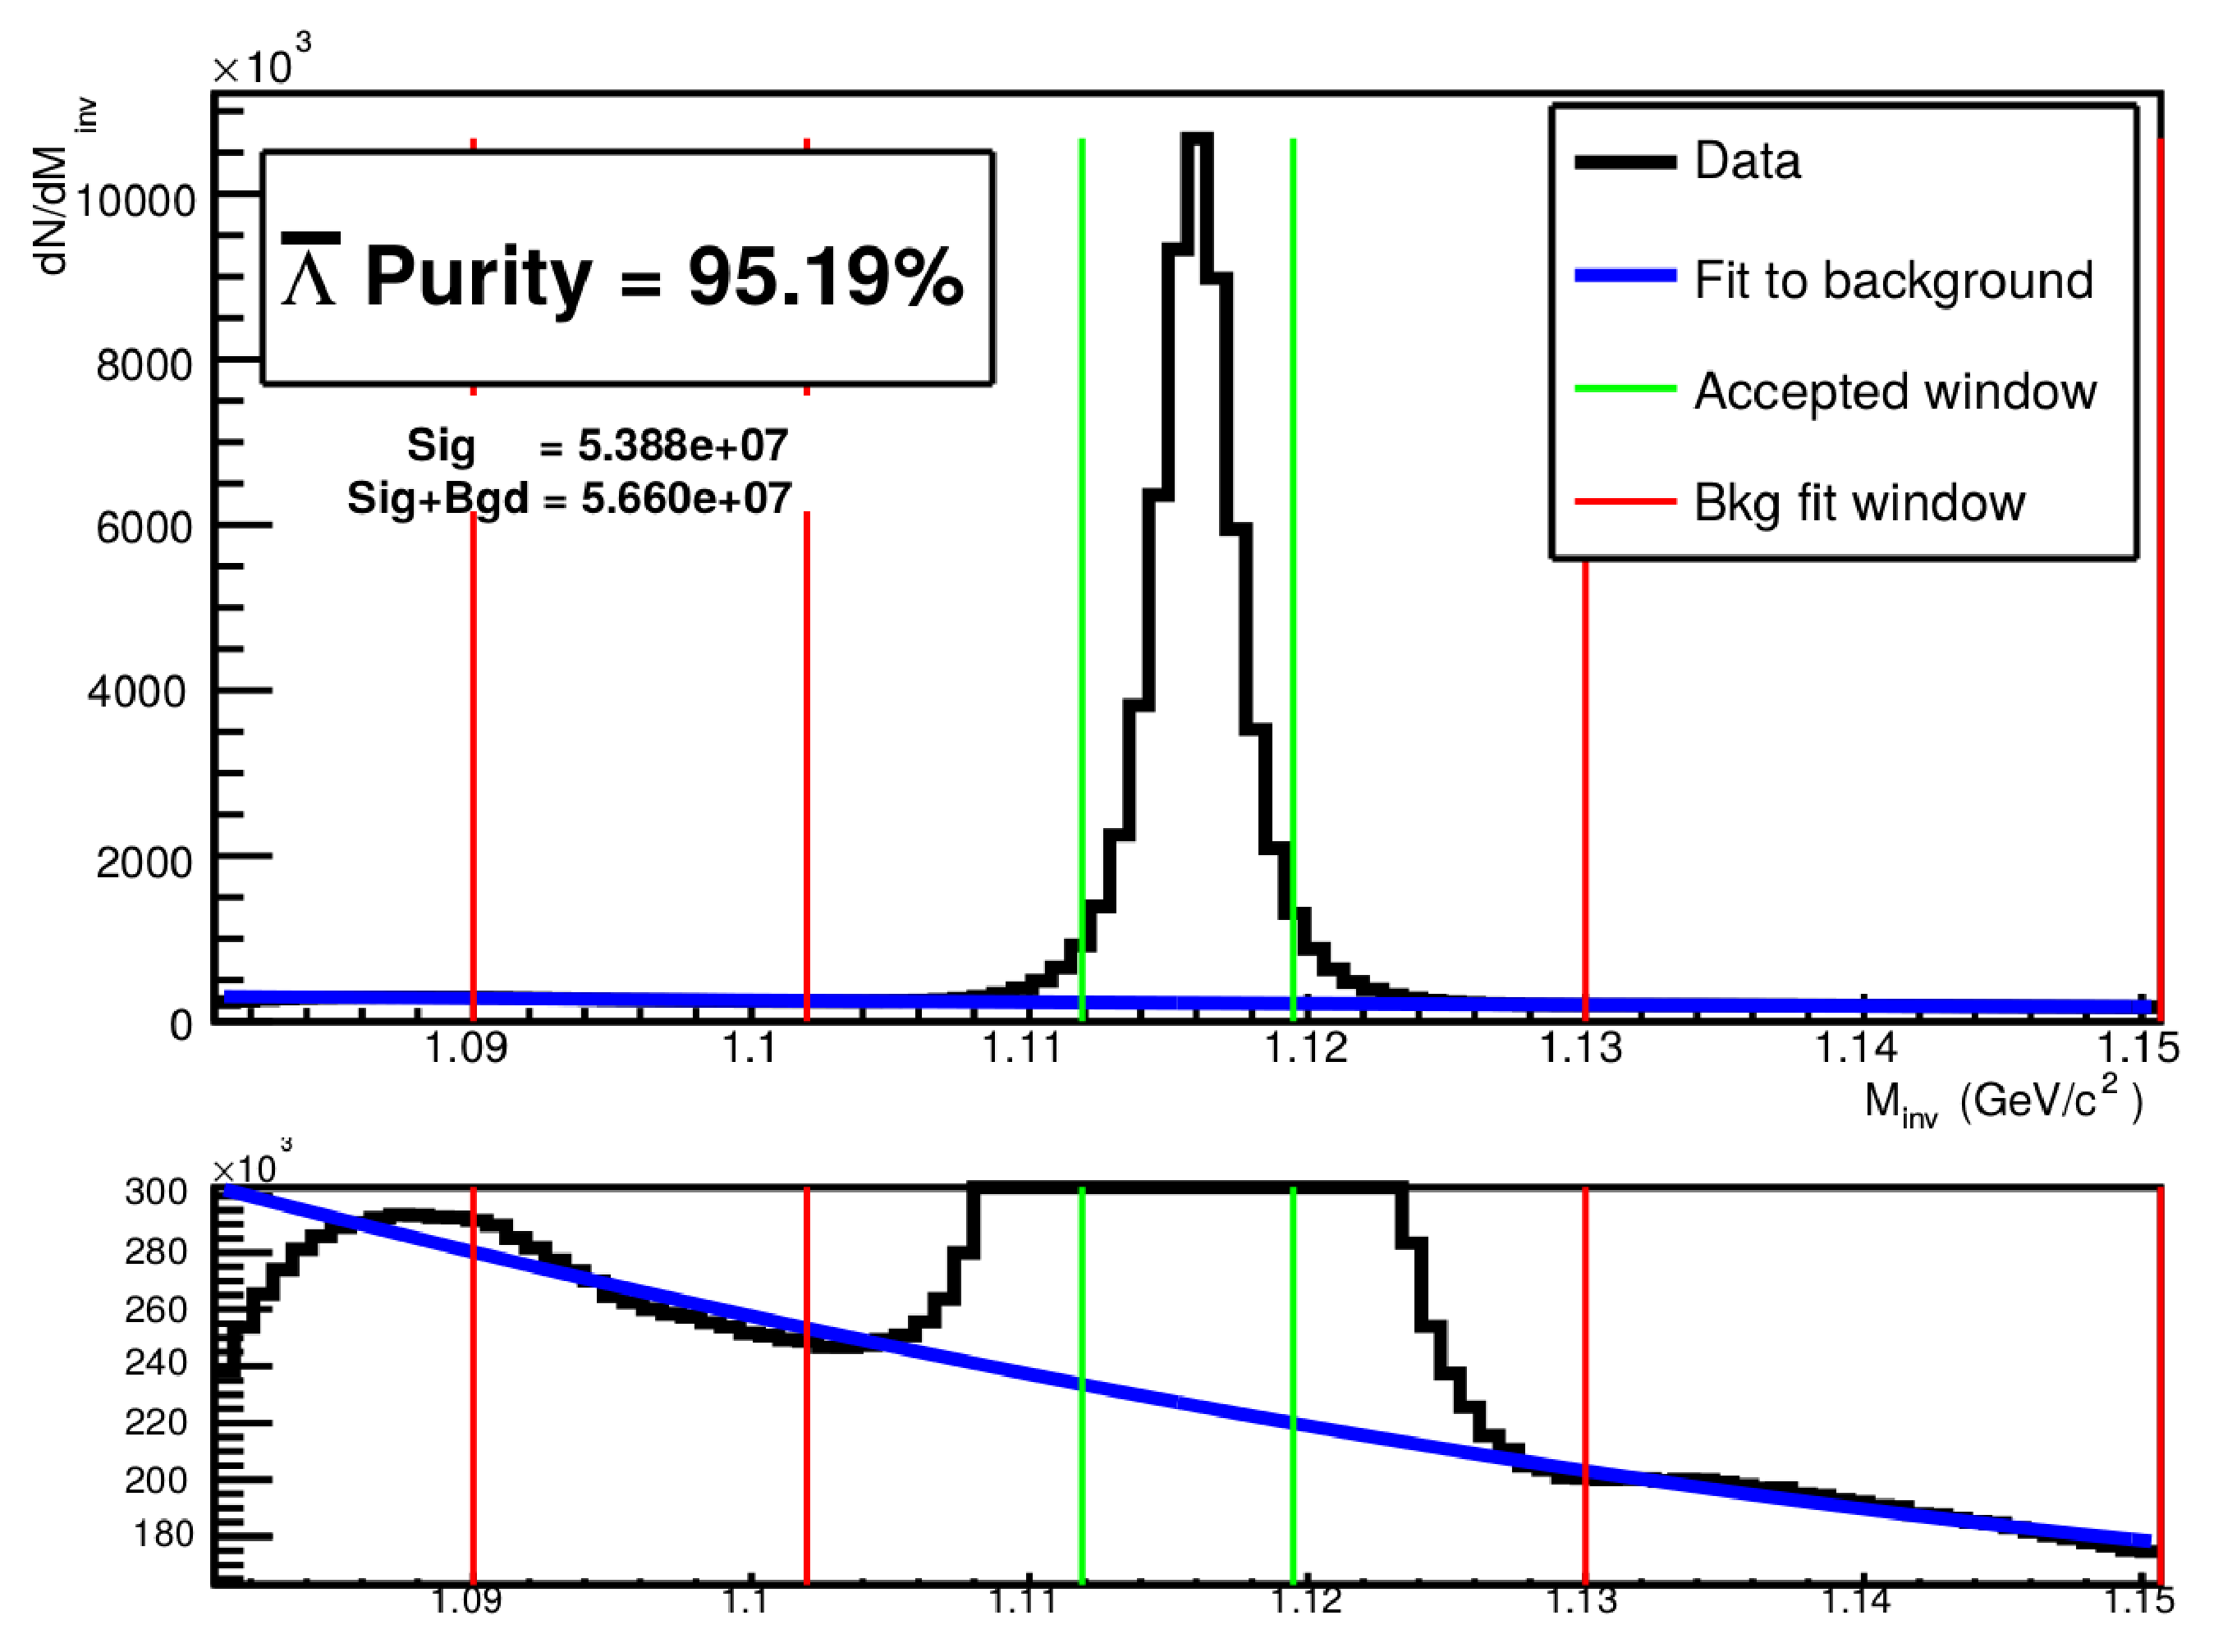
\includegraphics[width=0.49\textwidth]{/home/jesse/Analysis/FemtoAnalysis/AnalysisNotes/3_DataSelection/Figures/ALamPurity_LamKch_0010.pdf}}
  %%----start of third subfigure---
  \\
  \subfloat[\LamKs Purity]{
    \label{fig:K0sPurity}
    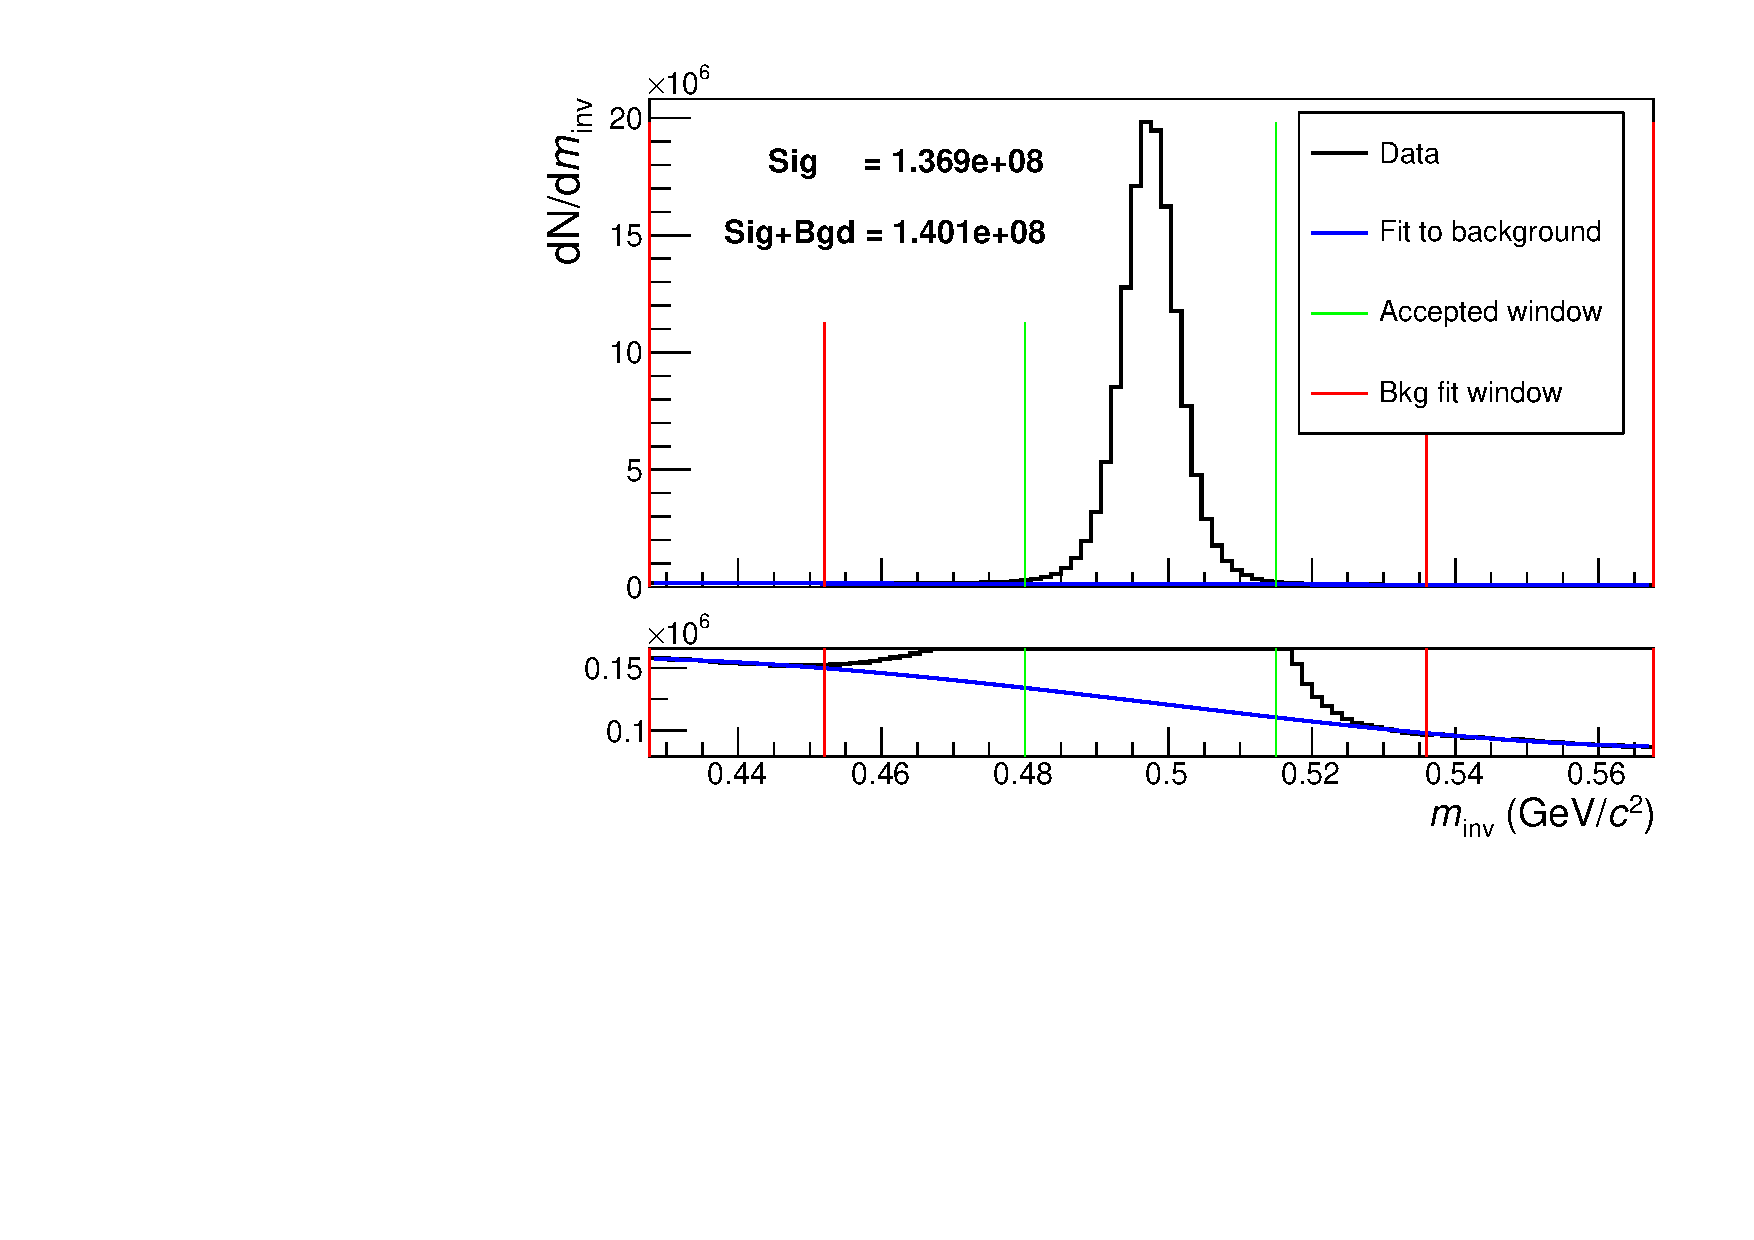
\includegraphics[width=0.49\textwidth]{/home/jesse/Analysis/FemtoAnalysis/AnalysisNotes/3_DataSelection/Figures/K0Purity_LamK0.pdf}}    
  %%----overall caption----
  \caption[V0 (\Lam, \ALam, \Ks) Purities]{Invariant mass (\minv) distribution for all \Lam (a), \ALam (b), and \Ks (c) candidates immediately before the final invariant mass cut.  The bottom figures are zoomed to show the background with fit.  The vertical green lines represent the \minv cuts used in the analyses, the red vertical lines delineate the regions over which the background was fit, and the blue line shows the background fit.  These distributions are used to calculate the collection purities, Purity(\Lam) $\approx$ Purity(\ALam) $\approx$ 95\%, and Purity(\Ks) $\approx$ 98\%.}
  \label{fig:Purities}
\end{figure}

\end{document}